\documentclass[1p]{elsarticle_modified}
%\bibliographystyle{elsarticle-num}

%\usepackage[colorlinks]{hyperref}
%\usepackage{abbrmath_seonhwa} %\Abb, \Ascr, \Acal ,\Abf, \Afrak
\usepackage{amsfonts}
\usepackage{amssymb}
\usepackage{amsmath}
\usepackage{amsthm}
\usepackage{scalefnt}
\usepackage{amsbsy}
\usepackage{kotex}
\usepackage{caption}
\usepackage{subfig}
\usepackage{color}
\usepackage{graphicx}
\usepackage{xcolor} %% white, black, red, green, blue, cyan, magenta, yellow
\usepackage{float}
\usepackage{setspace}
\usepackage{hyperref}

\usepackage{tikz}
\usetikzlibrary{arrows}

\usepackage{multirow}
\usepackage{array} % fixed length table
\usepackage{hhline}

%%%%%%%%%%%%%%%%%%%%%
\makeatletter
\renewcommand*\env@matrix[1][\arraystretch]{%
	\edef\arraystretch{#1}%
	\hskip -\arraycolsep
	\let\@ifnextchar\new@ifnextchar
	\array{*\c@MaxMatrixCols c}}
\makeatother %https://tex.stackexchange.com/questions/14071/how-can-i-increase-the-line-spacing-in-a-matrix
%%%%%%%%%%%%%%%

\usepackage[normalem]{ulem}

\newcommand{\msout}[1]{\ifmmode\text{\sout{\ensuremath{#1}}}\else\sout{#1}\fi}
%SOURCE: \msout is \stkout macro in https://tex.stackexchange.com/questions/20609/strikeout-in-math-mode

\newcommand{\cancel}[1]{
	\ifmmode
	{\color{red}\msout{#1}}
	\else
	{\color{red}\sout{#1}}
	\fi
}

\newcommand{\add}[1]{
	{\color{blue}\uwave{#1}}
}

\newcommand{\replace}[2]{
	\ifmmode
	{\color{red}\msout{#1}}{\color{blue}\uwave{#2}}
	\else
	{\color{red}\sout{#1}}{\color{blue}\uwave{#2}}
	\fi
}

\newcommand{\Sol}{\mathcal{S}} %segment
\newcommand{\D}{D} %diagram
\newcommand{\A}{\mathcal{A}} %arc


%%%%%%%%%%%%%%%%%%%%%%%%%%%%%5 test

\def\sl{\operatorname{\textup{SL}}(2,\Cbb)}
\def\psl{\operatorname{\textup{PSL}}(2,\Cbb)}
\def\quan{\mkern 1mu \triangleright \mkern 1mu}

\theoremstyle{definition}
\newtheorem{thm}{Theorem}[section]
\newtheorem{prop}[thm]{Proposition}
\newtheorem{lem}[thm]{Lemma}
\newtheorem{ques}[thm]{Question}
\newtheorem{cor}[thm]{Corollary}
\newtheorem{defn}[thm]{Definition}
\newtheorem{exam}[thm]{Example}
\newtheorem{rmk}[thm]{Remark}
\newtheorem{alg}[thm]{Algorithm}

\newcommand{\I}{\sqrt{-1}}
\begin{document}

%\begin{frontmatter}
%
%\title{Boundary parabolic representations of knots up to 8 crossings}
%
%%% Group authors per affiliation:
%\author{Yunhi Cho} 
%\address{Department of Mathematics, University of Seoul, Seoul, Korea}
%\ead{yhcho@uos.ac.kr}
%
%
%\author{Seonhwa Kim} %\fnref{s_kim}}
%\address{Center for Geometry and Physics, Institute for Basic Science, Pohang, 37673, Korea}
%\ead{ryeona17@ibs.re.kr}
%
%\author{Hyuk Kim}
%\address{Department of Mathematical Sciences, Seoul National University, Seoul 08826, Korea}
%\ead{hyukkim@snu.ac.kr}
%
%\author{Seokbeom Yoon}
%\address{Department of Mathematical Sciences, Seoul National University, Seoul, 08826,  Korea}
%\ead{sbyoon15@snu.ac.kr}
%
%\begin{abstract}
%We find all boundary parabolic representation of knots up to 8 crossings.
%
%\end{abstract}
%\begin{keyword}
%    \MSC[2010] 57M25 
%\end{keyword}
%
%\end{frontmatter}

%\linenumbers
%\tableofcontents
%
\newcommand\colored[1]{\textcolor{white}{\rule[-0.35ex]{0.8em}{1.4ex}}\kern-0.8em\color{red} #1}%
%\newcommand\colored[1]{\textcolor{white}{ #1}\kern-2.17ex	\textcolor{white}{ #1}\kern-1.81ex	\textcolor{white}{ #1}\kern-2.15ex\color{red}#1	}

{\Large $\underline{11a_{194}~(K11a_{194})}$}

\setlength{\tabcolsep}{10pt}
\renewcommand{\arraystretch}{1.6}
\vspace{1cm}\begin{tabular}{m{100pt}>{\centering\arraybackslash}m{274pt}}
\multirow{5}{120pt}{
	\centering
	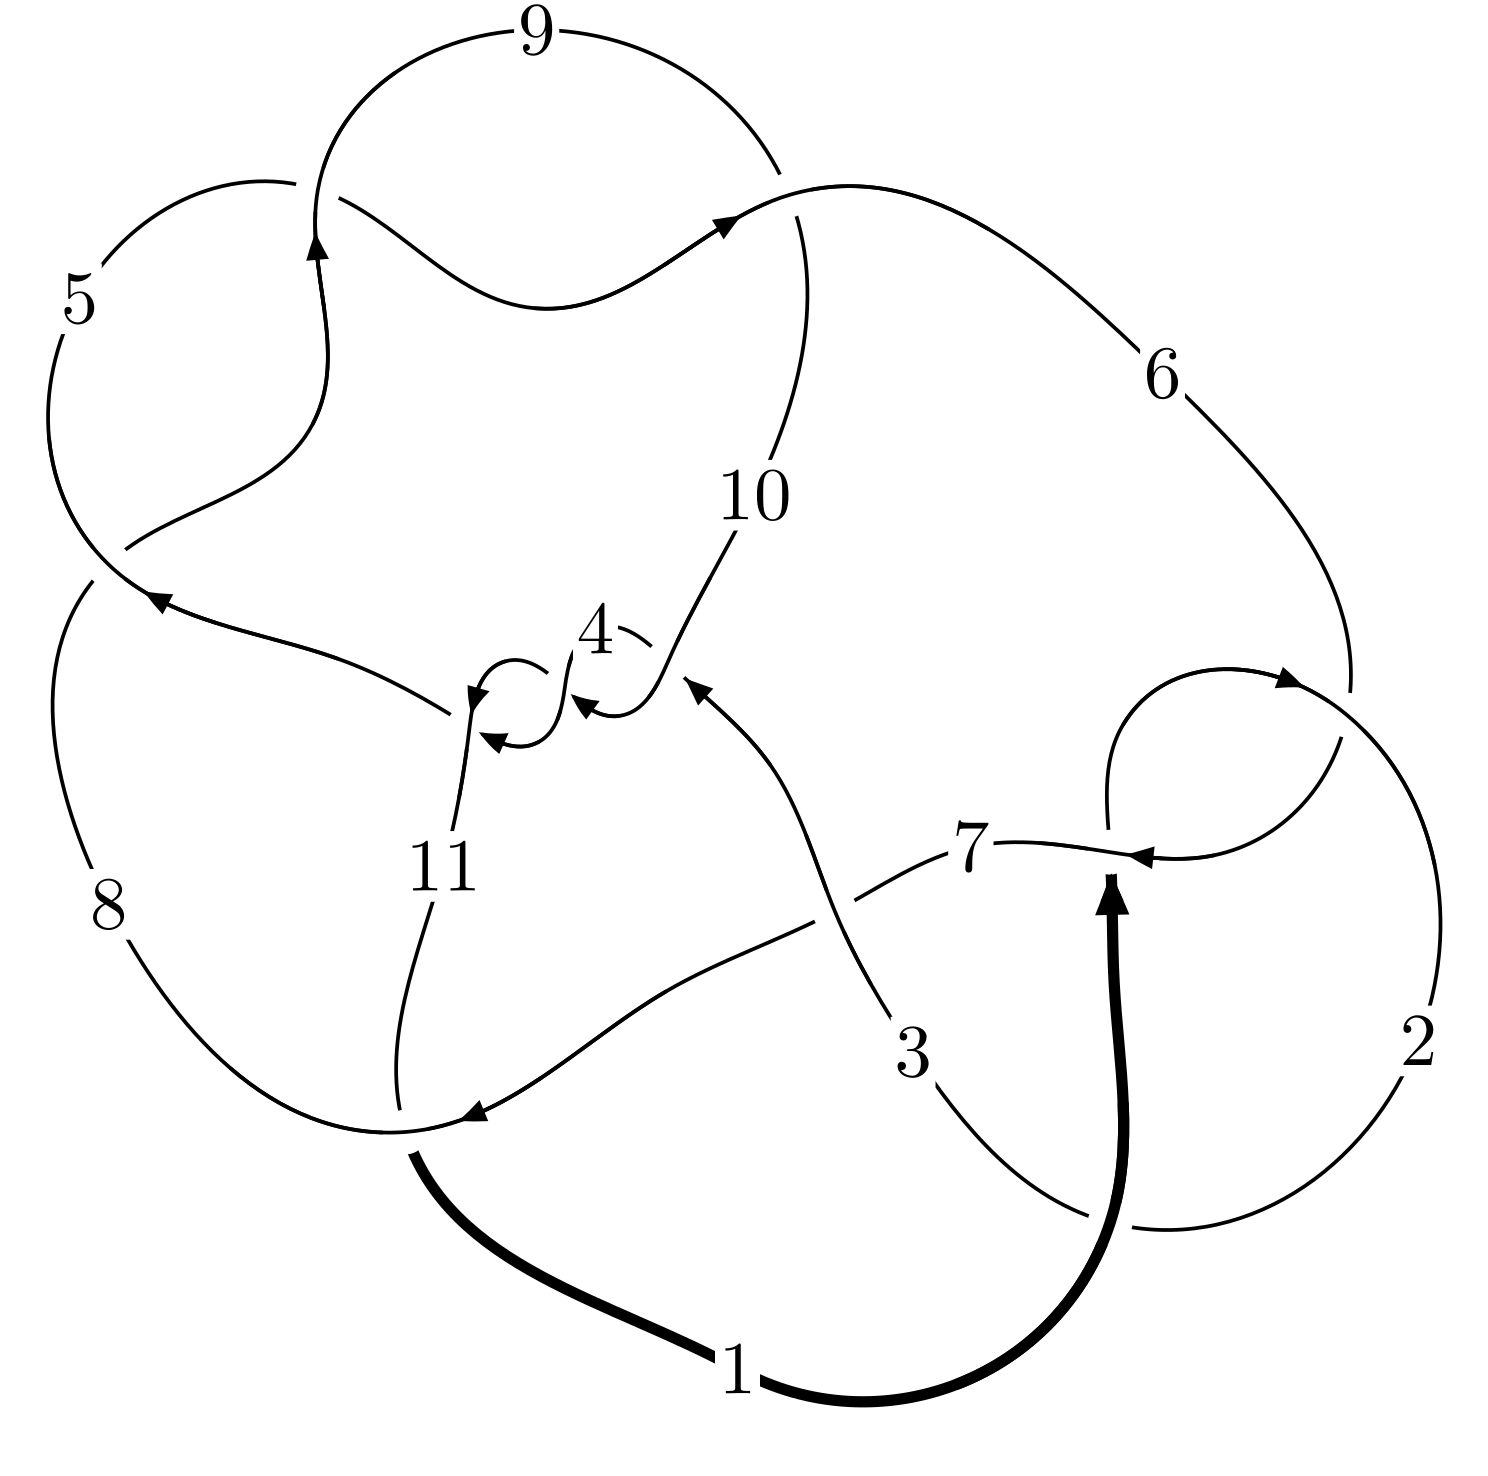
\includegraphics[width=112pt]{../../../GIT/diagram.site/Diagrams/png/443_11a_194.png}\\
\ \ \ A knot diagram\footnotemark}&
\allowdisplaybreaks
\textbf{Linearized knot diagam} \\
\cline{2-2}
 &
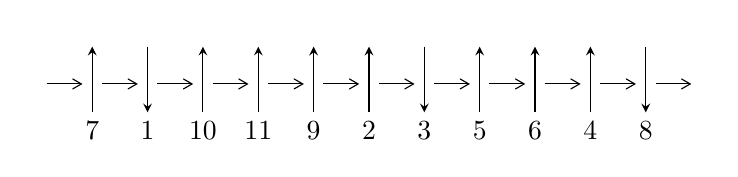
\begin{tikzpicture}[x=20pt, y=17pt]
	% nodes
	\node (C0) at (0, 0) {};
	\node (C1) at (1, 0) {};
	\node (C1U) at (1, +1) {};
	\node (C1D) at (1, -1) {7};

	\node (C2) at (2, 0) {};
	\node (C2U) at (2, +1) {};
	\node (C2D) at (2, -1) {1};

	\node (C3) at (3, 0) {};
	\node (C3U) at (3, +1) {};
	\node (C3D) at (3, -1) {10};

	\node (C4) at (4, 0) {};
	\node (C4U) at (4, +1) {};
	\node (C4D) at (4, -1) {11};

	\node (C5) at (5, 0) {};
	\node (C5U) at (5, +1) {};
	\node (C5D) at (5, -1) {9};

	\node (C6) at (6, 0) {};
	\node (C6U) at (6, +1) {};
	\node (C6D) at (6, -1) {2};

	\node (C7) at (7, 0) {};
	\node (C7U) at (7, +1) {};
	\node (C7D) at (7, -1) {3};

	\node (C8) at (8, 0) {};
	\node (C8U) at (8, +1) {};
	\node (C8D) at (8, -1) {5};

	\node (C9) at (9, 0) {};
	\node (C9U) at (9, +1) {};
	\node (C9D) at (9, -1) {6};

	\node (C10) at (10, 0) {};
	\node (C10U) at (10, +1) {};
	\node (C10D) at (10, -1) {4};

	\node (C11) at (11, 0) {};
	\node (C11U) at (11, +1) {};
	\node (C11D) at (11, -1) {8};
	\node (C12) at (12, 0) {};

	% arrows
	\draw[->,>={angle 60}]
	(C0) edge (C1) (C1) edge (C2) (C2) edge (C3) (C3) edge (C4) (C4) edge (C5) (C5) edge (C6) (C6) edge (C7) (C7) edge (C8) (C8) edge (C9) (C9) edge (C10) (C10) edge (C11) (C11) edge (C12) ;	\draw[->,>=stealth]
	(C1D) edge (C1U) (C2U) edge (C2D) (C3D) edge (C3U) (C4D) edge (C4U) (C5D) edge (C5U) (C6D) edge (C6U) (C7U) edge (C7D) (C8D) edge (C8U) (C9D) edge (C9U) (C10D) edge (C10U) (C11U) edge (C11D) ;
	\end{tikzpicture} \\
\hhline{~~} \\& 
\textbf{Solving Sequence} \\ \cline{2-2} 
 &
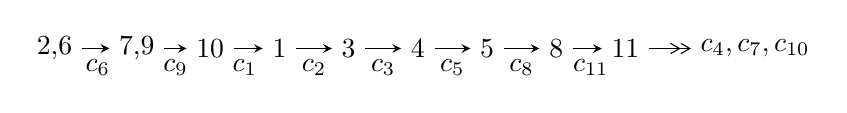
\begin{tikzpicture}[x=25pt, y=7pt]
	% node
	\node (A0) at (-1/8, 0) {2,6};
	\node (A1) at (17/16, 0) {7,9};
	\node (A2) at (17/8, 0) {10};
	\node (A3) at (25/8, 0) {1};
	\node (A4) at (33/8, 0) {3};
	\node (A5) at (41/8, 0) {4};
	\node (A6) at (49/8, 0) {5};
	\node (A7) at (57/8, 0) {8};
	\node (A8) at (65/8, 0) {11};
	\node (C1) at (1/2, -1) {$c_{6}$};
	\node (C2) at (13/8, -1) {$c_{9}$};
	\node (C3) at (21/8, -1) {$c_{1}$};
	\node (C4) at (29/8, -1) {$c_{2}$};
	\node (C5) at (37/8, -1) {$c_{3}$};
	\node (C6) at (45/8, -1) {$c_{5}$};
	\node (C7) at (53/8, -1) {$c_{8}$};
	\node (C8) at (61/8, -1) {$c_{11}$};
	\node (A9) at (10, 0) {$c_{4},c_{7},c_{10}$};

	% edge
	\draw[->,>=stealth]	
	(A0) edge (A1) (A1) edge (A2) (A2) edge (A3) (A3) edge (A4) (A4) edge (A5) (A5) edge (A6) (A6) edge (A7) (A7) edge (A8) ;
	\draw[->>,>={angle 60}]	
	(A8) edge (A9);
\end{tikzpicture} \\ 

\end{tabular} \\

\footnotetext{
The image of knot diagram is generated by the software ``\textbf{Draw programme}" developed by Andrew Bartholomew(\url{http://www.layer8.co.uk/maths/draw/index.htm\#Running-draw}), where we modified some parts for our purpose(\url{https://github.com/CATsTAILs/LinksPainter}).
}\phantom \\ \newline 
\centering \textbf{Ideals for irreducible components\footnotemark of $X_{\text{par}}$} 
 
\begin{align*}
I^u_{1}&=\langle 
u^{22}-2 u^{21}+\cdots+b+1,\;3 u^{22}-7 u^{21}+\cdots+2 a-8 u,\;u^{23}-3 u^{22}+\cdots+6 u-2\rangle \\
I^u_{2}&=\langle 
-26 u^{14} a+25 u^{14}+\cdots-45 a+53,\;u^{14}+2 u^{13}+\cdots-2 a+2,\\
\phantom{I^u_{2}}&\phantom{= \langle  }u^{15}+u^{14}+4 u^{13}+3 u^{12}+8 u^{11}+6 u^{10}+10 u^9+7 u^8+8 u^7+6 u^6+6 u^5+4 u^4+4 u^3+2 u^2+2 u+1\rangle \\
I^u_{3}&=\langle 
b-1,\;u^3-2 u^2+2 a-2,\;u^4+2 u^2+2\rangle \\
\\
I^v_{1}&=\langle 
a,\;b+1,\;v+1\rangle \\
\end{align*}
\raggedright * 4 irreducible components of $\dim_{\mathbb{C}}=0$, with total 58 representations.\\
\footnotetext{All coefficients of polynomials are rational numbers. But the coefficients are sometimes approximated in decimal forms when there is not enough margin.}
\newpage
\renewcommand{\arraystretch}{1}
\centering \section*{I. $I^u_{1}= \langle u^{22}-2 u^{21}+\cdots+b+1,\;3 u^{22}-7 u^{21}+\cdots+2 a-8 u,\;u^{23}-3 u^{22}+\cdots+6 u-2 \rangle$}
\flushleft \textbf{(i) Arc colorings}\\
\begin{tabular}{m{7pt} m{180pt} m{7pt} m{180pt} }
\flushright $a_{2}=$&$\begin{pmatrix}0\\u\end{pmatrix}$ \\
\flushright $a_{6}=$&$\begin{pmatrix}1\\0\end{pmatrix}$ \\
\flushright $a_{7}=$&$\begin{pmatrix}1\\- u^2\end{pmatrix}$ \\
\flushright $a_{9}=$&$\begin{pmatrix}-\frac{3}{2} u^{22}+\frac{7}{2} u^{21}+\cdots-7 u^2+4 u\\- u^{22}+2 u^{21}+\cdots+2 u-1\end{pmatrix}$ \\
\flushright $a_{10}=$&$\begin{pmatrix}-\frac{5}{2} u^{22}+\frac{11}{2} u^{21}+\cdots+6 u-1\\- u^{22}+2 u^{21}+\cdots+2 u-1\end{pmatrix}$ \\
\flushright $a_{1}=$&$\begin{pmatrix}- u\\u^3+u\end{pmatrix}$ \\
\flushright $a_{3}=$&$\begin{pmatrix}- u^3\\u^5+u^3+u\end{pmatrix}$ \\
\flushright $a_{4}=$&$\begin{pmatrix}-\frac{1}{2} u^{22}+\frac{3}{2} u^{21}+\cdots+2 u-1\\u^{20}- u^{19}+\cdots- u+1\end{pmatrix}$ \\
\flushright $a_{5}=$&$\begin{pmatrix}-\frac{1}{2} u^{22}+\frac{3}{2} u^{21}+\cdots+4 u-1\\u^{20}- u^{19}+\cdots-2 u+1\end{pmatrix}$ \\
\flushright $a_{8}=$&$\begin{pmatrix}- u^6- u^4+1\\u^8+2 u^6+2 u^4\end{pmatrix}$ \\
\flushright $a_{11}=$&$\begin{pmatrix}- u^{11}-2 u^9-2 u^7+u^3\\u^{13}+3 u^{11}+5 u^9+4 u^7+2 u^5+u^3+u\end{pmatrix}$\\ \flushright $a_{11}=$&$\begin{pmatrix}- u^{11}-2 u^9-2 u^7+u^3\\u^{13}+3 u^{11}+5 u^9+4 u^7+2 u^5+u^3+u\end{pmatrix}$\\&\end{tabular}
\flushleft \textbf{(ii) Obstruction class $= -1$}\\~\\
\flushleft \textbf{(iii) Cusp Shapes $= 2 u^{22}-6 u^{21}+18 u^{20}-32 u^{19}+58 u^{18}-84 u^{17}+122 u^{16}-152 u^{15}+182 u^{14}-192 u^{13}+206 u^{12}-194 u^{11}+188 u^{10}-154 u^9+126 u^8-102 u^7+68 u^6-38 u^5+12 u^4+6 u^3+8 u^2-2 u+4$}\\~\\
\newpage\renewcommand{\arraystretch}{1}
\flushleft \textbf{(iv) u-Polynomials at the component}\newline \\
\begin{tabular}{m{50pt}|m{274pt}}
Crossings & \hspace{64pt}u-Polynomials at each crossing \\
\hline $$\begin{aligned}c_{1},c_{6}\end{aligned}$$&$\begin{aligned}
&u^{23}+3 u^{22}+\cdots+6 u+2
\end{aligned}$\\
\hline $$\begin{aligned}c_{2}\end{aligned}$$&$\begin{aligned}
&u^{23}+11 u^{22}+\cdots-4 u-4
\end{aligned}$\\
\hline $$\begin{aligned}c_{3},c_{4},c_{5}\\c_{8},c_{9},c_{10}\end{aligned}$$&$\begin{aligned}
&u^{23}- u^{22}+\cdots+4 u^2-1
\end{aligned}$\\
\hline $$\begin{aligned}c_{7}\end{aligned}$$&$\begin{aligned}
&u^{23}-3 u^{22}+\cdots-166 u+34
\end{aligned}$\\
\hline $$\begin{aligned}c_{11}\end{aligned}$$&$\begin{aligned}
&u^{23}+15 u^{22}+\cdots+1790 u+314
\end{aligned}$\\
\hline
\end{tabular}\\~\\
\newpage\renewcommand{\arraystretch}{1}
\flushleft \textbf{(v) Riley Polynomials at the component}\newline \\
\begin{tabular}{m{50pt}|m{274pt}}
Crossings & \hspace{64pt}Riley Polynomials at each crossing \\
\hline $$\begin{aligned}c_{1},c_{6}\end{aligned}$$&$\begin{aligned}
&y^{23}+11 y^{22}+\cdots-4 y-4
\end{aligned}$\\
\hline $$\begin{aligned}c_{2}\end{aligned}$$&$\begin{aligned}
&y^{23}+3 y^{22}+\cdots-208 y-16
\end{aligned}$\\
\hline $$\begin{aligned}c_{3},c_{4},c_{5}\\c_{8},c_{9},c_{10}\end{aligned}$$&$\begin{aligned}
&y^{23}-29 y^{22}+\cdots+8 y-1
\end{aligned}$\\
\hline $$\begin{aligned}c_{7}\end{aligned}$$&$\begin{aligned}
&y^{23}-5 y^{22}+\cdots+4028 y-1156
\end{aligned}$\\
\hline $$\begin{aligned}c_{11}\end{aligned}$$&$\begin{aligned}
&y^{23}+7 y^{22}+\cdots-489796 y-98596
\end{aligned}$\\
\hline
\end{tabular}\\~\\
\newpage\flushleft \textbf{(vi) Complex Volumes and Cusp Shapes}
$$\begin{array}{c|c|c}  
\text{Solutions to }I^u_{1}& \I (\text{vol} + \sqrt{-1}CS) & \text{Cusp shape}\\
 \hline 
\begin{aligned}
u &= -0.768464 + 0.625797 I \\
a &= -2.35900 - 0.70924 I \\
b &= \phantom{-}1.59436 - 0.22254 I\end{aligned}
 & \phantom{-}14.4326 - 5.1937 I & \phantom{-}13.7476 + 3.5950 I \\ \hline\begin{aligned}
u &= -0.768464 - 0.625797 I \\
a &= -2.35900 + 0.70924 I \\
b &= \phantom{-}1.59436 + 0.22254 I\end{aligned}
 & \phantom{-}14.4326 + 5.1937 I & \phantom{-}13.7476 - 3.5950 I \\ \hline\begin{aligned}
u &= \phantom{-}0.835379 + 0.384998 I \\
a &= -2.06431 - 0.48967 I \\
b &= \phantom{-}1.55191 - 0.30830 I\end{aligned}
 & \phantom{-}13.0517 - 8.4231 I & \phantom{-}12.86699 + 3.68057 I \\ \hline\begin{aligned}
u &= \phantom{-}0.835379 - 0.384998 I \\
a &= -2.06431 + 0.48967 I \\
b &= \phantom{-}1.55191 + 0.30830 I\end{aligned}
 & \phantom{-}13.0517 + 8.4231 I & \phantom{-}12.86699 - 3.68057 I \\ \hline\begin{aligned}
u &= \phantom{-}0.305961 + 1.048060 I \\
a &= \phantom{-}0.143181 - 0.764944 I \\
b &= \phantom{-}0.168196 - 0.598689 I\end{aligned}
 & -3.26008 + 0.62293 I & -1.92583 + 0.88926 I \\ \hline\begin{aligned}
u &= \phantom{-}0.305961 - 1.048060 I \\
a &= \phantom{-}0.143181 + 0.764944 I \\
b &= \phantom{-}0.168196 + 0.598689 I\end{aligned}
 & -3.26008 - 0.62293 I & -1.92583 - 0.88926 I \\ \hline\begin{aligned}
u &= -0.477361 + 1.058390 I \\
a &= -0.325021 - 0.446372 I \\
b &= \phantom{-}0.496916 + 0.116873 I\end{aligned}
 & -0.90872 - 3.31162 I & \phantom{-}4.18007 + 2.04912 I \\ \hline\begin{aligned}
u &= -0.477361 - 1.058390 I \\
a &= -0.325021 + 0.446372 I \\
b &= \phantom{-}0.496916 - 0.116873 I\end{aligned}
 & -0.90872 + 3.31162 I & \phantom{-}4.18007 - 2.04912 I \\ \hline\begin{aligned}
u &= -0.666288 + 0.980877 I \\
a &= \phantom{-}1.51895 + 1.19962 I \\
b &= -1.60630 - 0.17413 I\end{aligned}
 & \phantom{-}13.37540 - 0.20863 I & \phantom{-}12.34199 + 1.72313 I \\ \hline\begin{aligned}
u &= -0.666288 - 0.980877 I \\
a &= \phantom{-}1.51895 - 1.19962 I \\
b &= -1.60630 + 0.17413 I\end{aligned}
 & \phantom{-}13.37540 + 0.20863 I & \phantom{-}12.34199 - 1.72313 I\\
 \hline 
 \end{array}$$\newpage$$\begin{array}{c|c|c}  
\text{Solutions to }I^u_{1}& \I (\text{vol} + \sqrt{-1}CS) & \text{Cusp shape}\\
 \hline 
\begin{aligned}
u &= \phantom{-}0.810177\phantom{ +0.000000I} \\
a &= \phantom{-}1.05047\phantom{ +0.000000I} \\
b &= -1.45269\phantom{ +0.000000I}\end{aligned}
 & \phantom{-}7.53068\phantom{ +0.000000I} & \phantom{-}12.4950\phantom{ +0.000000I} \\ \hline\begin{aligned}
u &= \phantom{-}0.150597 + 1.188510 I \\
a &= -0.209754 + 0.504264 I \\
b &= -1.50263 + 0.26695 I\end{aligned}
 & \phantom{-}7.74907 - 5.71311 I & \phantom{-}7.54100 + 2.76920 I \\ \hline\begin{aligned}
u &= \phantom{-}0.150597 - 1.188510 I \\
a &= -0.209754 - 0.504264 I \\
b &= -1.50263 - 0.26695 I\end{aligned}
 & \phantom{-}7.74907 + 5.71311 I & \phantom{-}7.54100 - 2.76920 I \\ \hline\begin{aligned}
u &= \phantom{-}0.534647 + 1.084890 I \\
a &= -1.091580 + 0.807678 I \\
b &= \phantom{-}0.370860 + 0.589443 I\end{aligned}
 & -1.70058 + 6.34697 I & \phantom{-}2.48807 - 8.83395 I \\ \hline\begin{aligned}
u &= \phantom{-}0.534647 - 1.084890 I \\
a &= -1.091580 - 0.807678 I \\
b &= \phantom{-}0.370860 - 0.589443 I\end{aligned}
 & -1.70058 - 6.34697 I & \phantom{-}2.48807 + 8.83395 I \\ \hline\begin{aligned}
u &= \phantom{-}0.432454 + 1.201200 I \\
a &= \phantom{-}0.317778 + 1.107100 I \\
b &= \phantom{-}1.412020 + 0.045870 I\end{aligned}
 & \phantom{-}3.91675 + 4.39214 I & \phantom{-}8.96484 - 3.62176 I \\ \hline\begin{aligned}
u &= \phantom{-}0.432454 - 1.201200 I \\
a &= \phantom{-}0.317778 - 1.107100 I \\
b &= \phantom{-}1.412020 - 0.045870 I\end{aligned}
 & \phantom{-}3.91675 - 4.39214 I & \phantom{-}8.96484 + 3.62176 I \\ \hline\begin{aligned}
u &= \phantom{-}0.624484 + 0.349425 I \\
a &= \phantom{-}0.805631 - 0.022305 I \\
b &= -0.341398 + 0.488155 I\end{aligned}
 & \phantom{-}0.39287 - 1.77603 I & \phantom{-}5.94653 + 5.32090 I \\ \hline\begin{aligned}
u &= \phantom{-}0.624484 - 0.349425 I \\
a &= \phantom{-}0.805631 + 0.022305 I \\
b &= -0.341398 - 0.488155 I\end{aligned}
 & \phantom{-}0.39287 + 1.77603 I & \phantom{-}5.94653 - 5.32090 I \\ \hline\begin{aligned}
u &= \phantom{-}0.609932 + 1.133500 I \\
a &= \phantom{-}1.32397 - 2.18810 I \\
b &= -1.53955 - 0.33727 I\end{aligned}
 & \phantom{-}10.8121 + 13.7968 I & \phantom{-}9.98537 - 7.70704 I\\
 \hline 
 \end{array}$$\newpage$$\begin{array}{c|c|c}  
\text{Solutions to }I^u_{1}& \I (\text{vol} + \sqrt{-1}CS) & \text{Cusp shape}\\
 \hline 
\begin{aligned}
u &= \phantom{-}0.609932 - 1.133500 I \\
a &= \phantom{-}1.32397 + 2.18810 I \\
b &= -1.53955 + 0.33727 I\end{aligned}
 & \phantom{-}10.8121 - 13.7968 I & \phantom{-}9.98537 + 7.70704 I \\ \hline\begin{aligned}
u &= -0.486428 + 0.465014 I \\
a &= \phantom{-}0.914914 + 0.002129 I \\
b &= -0.378035 + 0.245051 I\end{aligned}
 & \phantom{-}0.881089 - 0.706259 I & \phantom{-}8.61582 + 5.28098 I \\ \hline\begin{aligned}
u &= -0.486428 - 0.465014 I \\
a &= \phantom{-}0.914914 - 0.002129 I \\
b &= -0.378035 - 0.245051 I\end{aligned}
 & \phantom{-}0.881089 + 0.706259 I & \phantom{-}8.61582 - 5.28098 I\\
 \hline 
 \end{array}$$\newpage\newpage\renewcommand{\arraystretch}{1}
\centering \section*{II. $I^u_{2}= \langle -26 u^{14} a+25 u^{14}+\cdots-45 a+53,\;u^{14}+2 u^{13}+\cdots-2 a+2,\;u^{15}+u^{14}+\cdots+2 u+1 \rangle$}
\flushleft \textbf{(i) Arc colorings}\\
\begin{tabular}{m{7pt} m{180pt} m{7pt} m{180pt} }
\flushright $a_{2}=$&$\begin{pmatrix}0\\u\end{pmatrix}$ \\
\flushright $a_{6}=$&$\begin{pmatrix}1\\0\end{pmatrix}$ \\
\flushright $a_{7}=$&$\begin{pmatrix}1\\- u^2\end{pmatrix}$ \\
\flushright $a_{9}=$&$\begin{pmatrix}a\\2.36364 a u^{14}-2.27273 u^{14}+\cdots+4.09091 a-4.81818\end{pmatrix}$ \\
\flushright $a_{10}=$&$\begin{pmatrix}2.36364 a u^{14}-2.27273 u^{14}+\cdots+5.09091 a-4.81818\\2.36364 a u^{14}-2.27273 u^{14}+\cdots+4.09091 a-4.81818\end{pmatrix}$ \\
\flushright $a_{1}=$&$\begin{pmatrix}- u\\u^3+u\end{pmatrix}$ \\
\flushright $a_{3}=$&$\begin{pmatrix}- u^3\\u^5+u^3+u\end{pmatrix}$ \\
\flushright $a_{4}=$&$\begin{pmatrix}-2.27273 a u^{14}+2.45455 u^{14}+\cdots-4.81818 a+4.36364\\-1\end{pmatrix}$ \\
\flushright $a_{5}=$&$\begin{pmatrix}2.27273 a u^{14}-2.45455 u^{14}+\cdots+4.81818 a-4.36364\\-1.81818 a u^{14}+2.36364 u^{14}+\cdots-3.45455 a+5.09091\end{pmatrix}$ \\
\flushright $a_{8}=$&$\begin{pmatrix}- u^6- u^4+1\\u^8+2 u^6+2 u^4\end{pmatrix}$ \\
\flushright $a_{11}=$&$\begin{pmatrix}- u^{11}-2 u^9-2 u^7+u^3\\u^{13}+3 u^{11}+5 u^9+4 u^7+2 u^5+u^3+u\end{pmatrix}$\\ \flushright $a_{11}=$&$\begin{pmatrix}- u^{11}-2 u^9-2 u^7+u^3\\u^{13}+3 u^{11}+5 u^9+4 u^7+2 u^5+u^3+u\end{pmatrix}$\\&\end{tabular}
\flushleft \textbf{(ii) Obstruction class $= -1$}\\~\\
\flushleft \textbf{(iii) Cusp Shapes $= -4 u^{13}-4 u^{12}-12 u^{11}-12 u^{10}-20 u^9-24 u^8-20 u^7-24 u^6-16 u^5-16 u^4-16 u^3-8 u^2-8 u+2$}\\~\\
\newpage\renewcommand{\arraystretch}{1}
\flushleft \textbf{(iv) u-Polynomials at the component}\newline \\
\begin{tabular}{m{50pt}|m{274pt}}
Crossings & \hspace{64pt}u-Polynomials at each crossing \\
\hline $$\begin{aligned}c_{1},c_{6}\end{aligned}$$&$\begin{aligned}
&(u^{15}- u^{14}+\cdots+2 u-1)^{2}
\end{aligned}$\\
\hline $$\begin{aligned}c_{2}\end{aligned}$$&$\begin{aligned}
&(u^{15}+7 u^{14}+\cdots+4 u^2-1)^{2}
\end{aligned}$\\
\hline $$\begin{aligned}c_{3},c_{4},c_{5}\\c_{8},c_{9},c_{10}\end{aligned}$$&$\begin{aligned}
&u^{30}- u^{29}+\cdots-6 u-1
\end{aligned}$\\
\hline $$\begin{aligned}c_{7}\end{aligned}$$&$\begin{aligned}
&(u^{15}+u^{14}+\cdots-4 u-1)^{2}
\end{aligned}$\\
\hline $$\begin{aligned}c_{11}\end{aligned}$$&$\begin{aligned}
&(u^{15}-5 u^{14}+\cdots+12 u^3-1)^{2}
\end{aligned}$\\
\hline
\end{tabular}\\~\\
\newpage\renewcommand{\arraystretch}{1}
\flushleft \textbf{(v) Riley Polynomials at the component}\newline \\
\begin{tabular}{m{50pt}|m{274pt}}
Crossings & \hspace{64pt}Riley Polynomials at each crossing \\
\hline $$\begin{aligned}c_{1},c_{6}\end{aligned}$$&$\begin{aligned}
&(y^{15}+7 y^{14}+\cdots+4 y^2-1)^{2}
\end{aligned}$\\
\hline $$\begin{aligned}c_{2}\end{aligned}$$&$\begin{aligned}
&(y^{15}+3 y^{14}+\cdots+8 y-1)^{2}
\end{aligned}$\\
\hline $$\begin{aligned}c_{3},c_{4},c_{5}\\c_{8},c_{9},c_{10}\end{aligned}$$&$\begin{aligned}
&y^{30}-25 y^{29}+\cdots+8 y+1
\end{aligned}$\\
\hline $$\begin{aligned}c_{7}\end{aligned}$$&$\begin{aligned}
&(y^{15}- y^{14}+\cdots+16 y-1)^{2}
\end{aligned}$\\
\hline $$\begin{aligned}c_{11}\end{aligned}$$&$\begin{aligned}
&(y^{15}+11 y^{14}+\cdots-84 y^2-1)^{2}
\end{aligned}$\\
\hline
\end{tabular}\\~\\
\newpage\flushleft \textbf{(vi) Complex Volumes and Cusp Shapes}
$$\begin{array}{c|c|c}  
\text{Solutions to }I^u_{2}& \I (\text{vol} + \sqrt{-1}CS) & \text{Cusp shape}\\
 \hline 
\begin{aligned}
u &= \phantom{-}0.385605 + 0.867795 I \\
a &= \phantom{-}1.48418 + 0.28748 I \\
b &= -1.191720 + 0.191378 I\end{aligned}
 & \phantom{-}2.93870 + 1.66084 I & \phantom{-}9.51042 - 3.96405 I \\ \hline\begin{aligned}
u &= \phantom{-}0.385605 + 0.867795 I \\
a &= -0.57671 + 2.31540 I \\
b &= \phantom{-}0.987326 + 0.341266 I\end{aligned}
 & \phantom{-}2.93870 + 1.66084 I & \phantom{-}9.51042 - 3.96405 I \\ \hline\begin{aligned}
u &= \phantom{-}0.385605 - 0.867795 I \\
a &= \phantom{-}1.48418 - 0.28748 I \\
b &= -1.191720 - 0.191378 I\end{aligned}
 & \phantom{-}2.93870 - 1.66084 I & \phantom{-}9.51042 + 3.96405 I \\ \hline\begin{aligned}
u &= \phantom{-}0.385605 - 0.867795 I \\
a &= -0.57671 - 2.31540 I \\
b &= \phantom{-}0.987326 - 0.341266 I\end{aligned}
 & \phantom{-}2.93870 - 1.66084 I & \phantom{-}9.51042 + 3.96405 I \\ \hline\begin{aligned}
u &= -0.146928 + 1.062740 I \\
a &= \phantom{-}0.506354 + 1.080350 I \\
b &= \phantom{-}0.417318 + 0.715805 I\end{aligned}
 & \phantom{-}1.46912 + 2.07402 I & \phantom{-}4.17178 - 2.67122 I \\ \hline\begin{aligned}
u &= -0.146928 + 1.062740 I \\
a &= \phantom{-}0.286056 - 0.497573 I \\
b &= -1.345540 - 0.160838 I\end{aligned}
 & \phantom{-}1.46912 + 2.07402 I & \phantom{-}4.17178 - 2.67122 I \\ \hline\begin{aligned}
u &= -0.146928 - 1.062740 I \\
a &= \phantom{-}0.506354 - 1.080350 I \\
b &= \phantom{-}0.417318 - 0.715805 I\end{aligned}
 & \phantom{-}1.46912 - 2.07402 I & \phantom{-}4.17178 + 2.67122 I \\ \hline\begin{aligned}
u &= -0.146928 - 1.062740 I \\
a &= \phantom{-}0.286056 + 0.497573 I \\
b &= -1.345540 + 0.160838 I\end{aligned}
 & \phantom{-}1.46912 - 2.07402 I & \phantom{-}4.17178 + 2.67122 I \\ \hline\begin{aligned}
u &= \phantom{-}0.715401 + 0.518352 I \\
a &= \phantom{-}0.929094 + 0.108337 I \\
b &= -0.681034 - 0.791319 I\end{aligned}
 & \phantom{-}6.82325 + 1.50523 I & \phantom{-}12.15133 - 2.74048 I \\ \hline\begin{aligned}
u &= \phantom{-}0.715401 + 0.518352 I \\
a &= -2.92853 + 0.30497 I \\
b &= \phantom{-}1.45955 + 0.03447 I\end{aligned}
 & \phantom{-}6.82325 + 1.50523 I & \phantom{-}12.15133 - 2.74048 I\\
 \hline 
 \end{array}$$\newpage$$\begin{array}{c|c|c}  
\text{Solutions to }I^u_{2}& \I (\text{vol} + \sqrt{-1}CS) & \text{Cusp shape}\\
 \hline 
\begin{aligned}
u &= \phantom{-}0.715401 - 0.518352 I \\
a &= \phantom{-}0.929094 - 0.108337 I \\
b &= -0.681034 + 0.791319 I\end{aligned}
 & \phantom{-}6.82325 - 1.50523 I & \phantom{-}12.15133 + 2.74048 I \\ \hline\begin{aligned}
u &= \phantom{-}0.715401 - 0.518352 I \\
a &= -2.92853 - 0.30497 I \\
b &= \phantom{-}1.45955 - 0.03447 I\end{aligned}
 & \phantom{-}6.82325 - 1.50523 I & \phantom{-}12.15133 + 2.74048 I \\ \hline\begin{aligned}
u &= -0.758945 + 0.422629 I \\
a &= \phantom{-}0.667191 + 0.185788 I \\
b &= -0.516053 - 0.873011 I\end{aligned}
 & \phantom{-}6.30676 + 4.09199 I & \phantom{-}11.04427 - 3.15094 I \\ \hline\begin{aligned}
u &= -0.758945 + 0.422629 I \\
a &= -2.63836 + 0.44671 I \\
b &= \phantom{-}1.46243 + 0.15596 I\end{aligned}
 & \phantom{-}6.30676 + 4.09199 I & \phantom{-}11.04427 - 3.15094 I \\ \hline\begin{aligned}
u &= -0.758945 - 0.422629 I \\
a &= \phantom{-}0.667191 - 0.185788 I \\
b &= -0.516053 + 0.873011 I\end{aligned}
 & \phantom{-}6.30676 - 4.09199 I & \phantom{-}11.04427 + 3.15094 I \\ \hline\begin{aligned}
u &= -0.758945 - 0.422629 I \\
a &= -2.63836 - 0.44671 I \\
b &= \phantom{-}1.46243 - 0.15596 I\end{aligned}
 & \phantom{-}6.30676 - 4.09199 I & \phantom{-}11.04427 + 3.15094 I \\ \hline\begin{aligned}
u &= -0.426893 + 1.085670 I \\
a &= -0.045925 - 1.153050 I \\
b &= \phantom{-}1.008860 - 0.127254 I\end{aligned}
 & -0.91830 - 3.60340 I & \phantom{-}1.83628 + 4.47672 I \\ \hline\begin{aligned}
u &= -0.426893 + 1.085670 I \\
a &= -0.652015 + 0.334121 I \\
b &= \phantom{-}0.026324 + 0.245041 I\end{aligned}
 & -0.91830 - 3.60340 I & \phantom{-}1.83628 + 4.47672 I \\ \hline\begin{aligned}
u &= -0.426893 - 1.085670 I \\
a &= -0.045925 + 1.153050 I \\
b &= \phantom{-}1.008860 + 0.127254 I\end{aligned}
 & -0.91830 + 3.60340 I & \phantom{-}1.83628 - 4.47672 I \\ \hline\begin{aligned}
u &= -0.426893 - 1.085670 I \\
a &= -0.652015 - 0.334121 I \\
b &= \phantom{-}0.026324 - 0.245041 I\end{aligned}
 & -0.91830 + 3.60340 I & \phantom{-}1.83628 - 4.47672 I\\
 \hline 
 \end{array}$$\newpage$$\begin{array}{c|c|c}  
\text{Solutions to }I^u_{2}& \I (\text{vol} + \sqrt{-1}CS) & \text{Cusp shape}\\
 \hline 
\begin{aligned}
u &= \phantom{-}0.594997 + 1.040830 I \\
a &= \phantom{-}0.400000 + 0.495676 I \\
b &= \phantom{-}0.773820 - 0.766183 I\end{aligned}
 & \phantom{-}5.27292 + 3.51852 I & \phantom{-}9.71302 - 2.59027 I \\ \hline\begin{aligned}
u &= \phantom{-}0.594997 + 1.040830 I \\
a &= \phantom{-}2.00079 - 1.63767 I \\
b &= -1.46460 - 0.02952 I\end{aligned}
 & \phantom{-}5.27292 + 3.51852 I & \phantom{-}9.71302 - 2.59027 I \\ \hline\begin{aligned}
u &= \phantom{-}0.594997 - 1.040830 I \\
a &= \phantom{-}0.400000 - 0.495676 I \\
b &= \phantom{-}0.773820 + 0.766183 I\end{aligned}
 & \phantom{-}5.27292 - 3.51852 I & \phantom{-}9.71302 + 2.59027 I \\ \hline\begin{aligned}
u &= \phantom{-}0.594997 - 1.040830 I \\
a &= \phantom{-}2.00079 + 1.63767 I \\
b &= -1.46460 + 0.02952 I\end{aligned}
 & \phantom{-}5.27292 - 3.51852 I & \phantom{-}9.71302 + 2.59027 I \\ \hline\begin{aligned}
u &= -0.594032 + 1.095620 I \\
a &= -1.24711 - 0.90132 I \\
b &= \phantom{-}0.463749 - 0.915832 I\end{aligned}
 & \phantom{-}4.31617 - 9.21780 I & \phantom{-}7.85460 + 7.39135 I \\ \hline\begin{aligned}
u &= -0.594032 + 1.095620 I \\
a &= \phantom{-}1.71287 + 2.15495 I \\
b &= -1.47039 + 0.20072 I\end{aligned}
 & \phantom{-}4.31617 - 9.21780 I & \phantom{-}7.85460 + 7.39135 I \\ \hline\begin{aligned}
u &= -0.594032 - 1.095620 I \\
a &= -1.24711 + 0.90132 I \\
b &= \phantom{-}0.463749 + 0.915832 I\end{aligned}
 & \phantom{-}4.31617 + 9.21780 I & \phantom{-}7.85460 - 7.39135 I \\ \hline\begin{aligned}
u &= -0.594032 - 1.095620 I \\
a &= \phantom{-}1.71287 - 2.15495 I \\
b &= -1.47039 - 0.20072 I\end{aligned}
 & \phantom{-}4.31617 + 9.21780 I & \phantom{-}7.85460 - 7.39135 I \\ \hline\begin{aligned}
u &= -0.538411\phantom{ +0.000000I} \\
a &= \phantom{-}1.00814\phantom{ +0.000000I} \\
b &= -1.09727\phantom{ +0.000000I}\end{aligned}
 & \phantom{-}1.86559\phantom{ +0.000000I} & \phantom{-}5.43660\phantom{ +0.000000I} \\ \hline\begin{aligned}
u &= -0.538411\phantom{ +0.000000I} \\
a &= \phantom{-}1.19609\phantom{ +0.000000I} \\
b &= \phantom{-}0.237195\phantom{ +0.000000I}\end{aligned}
 & \phantom{-}1.86559\phantom{ +0.000000I} & \phantom{-}5.43660\phantom{ +0.000000I}\\
 \hline 
 \end{array}$$\newpage\newpage\renewcommand{\arraystretch}{1}
\centering \section*{III. $I^u_{3}= \langle b-1,\;u^3-2 u^2+2 a-2,\;u^4+2 u^2+2 \rangle$}
\flushleft \textbf{(i) Arc colorings}\\
\begin{tabular}{m{7pt} m{180pt} m{7pt} m{180pt} }
\flushright $a_{2}=$&$\begin{pmatrix}0\\u\end{pmatrix}$ \\
\flushright $a_{6}=$&$\begin{pmatrix}1\\0\end{pmatrix}$ \\
\flushright $a_{7}=$&$\begin{pmatrix}1\\- u^2\end{pmatrix}$ \\
\flushright $a_{9}=$&$\begin{pmatrix}-\frac{1}{2} u^3+u^2+1\\1\end{pmatrix}$ \\
\flushright $a_{10}=$&$\begin{pmatrix}-\frac{1}{2} u^3+u^2+2\\1\end{pmatrix}$ \\
\flushright $a_{1}=$&$\begin{pmatrix}- u\\u^3+u\end{pmatrix}$ \\
\flushright $a_{3}=$&$\begin{pmatrix}- u^3\\- u^3- u\end{pmatrix}$ \\
\flushright $a_{4}=$&$\begin{pmatrix}-\frac{3}{2} u^3+u^2+2\\- u^3- u+1\end{pmatrix}$ \\
\flushright $a_{5}=$&$\begin{pmatrix}-\frac{1}{2} u^3+u^2+2\\1\end{pmatrix}$ \\
\flushright $a_{8}=$&$\begin{pmatrix}-1\\0\end{pmatrix}$ \\
\flushright $a_{11}=$&$\begin{pmatrix}u^3\\u^3+u\end{pmatrix}$\\ \flushright $a_{11}=$&$\begin{pmatrix}u^3\\u^3+u\end{pmatrix}$\\&\end{tabular}
\flushleft \textbf{(ii) Obstruction class $= 1$}\\~\\
\flushleft \textbf{(iii) Cusp Shapes $= -4 u^2+4$}\\~\\
\newpage\renewcommand{\arraystretch}{1}
\flushleft \textbf{(iv) u-Polynomials at the component}\newline \\
\begin{tabular}{m{50pt}|m{274pt}}
Crossings & \hspace{64pt}u-Polynomials at each crossing \\
\hline $$\begin{aligned}c_{1},c_{6}\end{aligned}$$&$\begin{aligned}
&u^4+2 u^2+2
\end{aligned}$\\
\hline $$\begin{aligned}c_{2}\end{aligned}$$&$\begin{aligned}
&(u^2+2 u+2)^2
\end{aligned}$\\
\hline $$\begin{aligned}c_{3},c_{4},c_{8}\\c_{9}\end{aligned}$$&$\begin{aligned}
&(u+1)^4
\end{aligned}$\\
\hline $$\begin{aligned}c_{5},c_{10}\end{aligned}$$&$\begin{aligned}
&(u-1)^4
\end{aligned}$\\
\hline $$\begin{aligned}c_{7},c_{11}\end{aligned}$$&$\begin{aligned}
&u^4-2 u^2+2
\end{aligned}$\\
\hline
\end{tabular}\\~\\
\newpage\renewcommand{\arraystretch}{1}
\flushleft \textbf{(v) Riley Polynomials at the component}\newline \\
\begin{tabular}{m{50pt}|m{274pt}}
Crossings & \hspace{64pt}Riley Polynomials at each crossing \\
\hline $$\begin{aligned}c_{1},c_{6}\end{aligned}$$&$\begin{aligned}
&(y^2+2 y+2)^2
\end{aligned}$\\
\hline $$\begin{aligned}c_{2}\end{aligned}$$&$\begin{aligned}
&(y^2+4)^2
\end{aligned}$\\
\hline $$\begin{aligned}c_{3},c_{4},c_{5}\\c_{8},c_{9},c_{10}\end{aligned}$$&$\begin{aligned}
&(y-1)^4
\end{aligned}$\\
\hline $$\begin{aligned}c_{7},c_{11}\end{aligned}$$&$\begin{aligned}
&(y^2-2 y+2)^2
\end{aligned}$\\
\hline
\end{tabular}\\~\\
\newpage\flushleft \textbf{(vi) Complex Volumes and Cusp Shapes}
$$\begin{array}{c|c|c}  
\text{Solutions to }I^u_{3}& \I (\text{vol} + \sqrt{-1}CS) & \text{Cusp shape}\\
 \hline 
\begin{aligned}
u &= \phantom{-}0.455090 + 1.098680 I \\
a &= \phantom{-}0.77689 + 1.32180 I \\
b &= \phantom{-}1.00000\phantom{ +0.000000I}\end{aligned}
 & \phantom{-}0.82247 + 3.66386 I & \phantom{-}8.00000 - 4.00000 I \\ \hline\begin{aligned}
u &= \phantom{-}0.455090 - 1.098680 I \\
a &= \phantom{-}0.77689 - 1.32180 I \\
b &= \phantom{-}1.00000\phantom{ +0.000000I}\end{aligned}
 & \phantom{-}0.82247 - 3.66386 I & \phantom{-}8.00000 + 4.00000 I \\ \hline\begin{aligned}
u &= -0.455090 + 1.098680 I \\
a &= -0.776887 - 0.678203 I \\
b &= \phantom{-}1.00000\phantom{ +0.000000I}\end{aligned}
 & \phantom{-}0.82247 - 3.66386 I & \phantom{-}8.00000 + 4.00000 I \\ \hline\begin{aligned}
u &= -0.455090 - 1.098680 I \\
a &= -0.776887 + 0.678203 I \\
b &= \phantom{-}1.00000\phantom{ +0.000000I}\end{aligned}
 & \phantom{-}0.82247 + 3.66386 I & \phantom{-}8.00000 - 4.00000 I\\
 \hline 
 \end{array}$$\newpage\newpage\renewcommand{\arraystretch}{1}
\centering \section*{IV. $I^v_{1}= \langle a,\;b+1,\;v+1 \rangle$}
\flushleft \textbf{(i) Arc colorings}\\
\begin{tabular}{m{7pt} m{180pt} m{7pt} m{180pt} }
\flushright $a_{2}=$&$\begin{pmatrix}-1\\0\end{pmatrix}$ \\
\flushright $a_{6}=$&$\begin{pmatrix}1\\0\end{pmatrix}$ \\
\flushright $a_{7}=$&$\begin{pmatrix}1\\0\end{pmatrix}$ \\
\flushright $a_{9}=$&$\begin{pmatrix}0\\-1\end{pmatrix}$ \\
\flushright $a_{10}=$&$\begin{pmatrix}-1\\-1\end{pmatrix}$ \\
\flushright $a_{1}=$&$\begin{pmatrix}-1\\0\end{pmatrix}$ \\
\flushright $a_{3}=$&$\begin{pmatrix}-1\\0\end{pmatrix}$ \\
\flushright $a_{4}=$&$\begin{pmatrix}0\\1\end{pmatrix}$ \\
\flushright $a_{5}=$&$\begin{pmatrix}1\\1\end{pmatrix}$ \\
\flushright $a_{8}=$&$\begin{pmatrix}1\\0\end{pmatrix}$ \\
\flushright $a_{11}=$&$\begin{pmatrix}-1\\0\end{pmatrix}$\\ \flushright $a_{11}=$&$\begin{pmatrix}-1\\0\end{pmatrix}$\\&\end{tabular}
\flushleft \textbf{(ii) Obstruction class $= 1$}\\~\\
\flushleft \textbf{(iii) Cusp Shapes $= 12$}\\~\\
\newpage\renewcommand{\arraystretch}{1}
\flushleft \textbf{(iv) u-Polynomials at the component}\newline \\
\begin{tabular}{m{50pt}|m{274pt}}
Crossings & \hspace{64pt}u-Polynomials at each crossing \\
\hline $$\begin{aligned}c_{1},c_{2},c_{6}\\c_{7},c_{11}\end{aligned}$$&$\begin{aligned}
&u
\end{aligned}$\\
\hline $$\begin{aligned}c_{3},c_{4},c_{8}\\c_{9}\end{aligned}$$&$\begin{aligned}
&u-1
\end{aligned}$\\
\hline $$\begin{aligned}c_{5},c_{10}\end{aligned}$$&$\begin{aligned}
&u+1
\end{aligned}$\\
\hline
\end{tabular}\\~\\
\newpage\renewcommand{\arraystretch}{1}
\flushleft \textbf{(v) Riley Polynomials at the component}\newline \\
\begin{tabular}{m{50pt}|m{274pt}}
Crossings & \hspace{64pt}Riley Polynomials at each crossing \\
\hline $$\begin{aligned}c_{1},c_{2},c_{6}\\c_{7},c_{11}\end{aligned}$$&$\begin{aligned}
&y
\end{aligned}$\\
\hline $$\begin{aligned}c_{3},c_{4},c_{5}\\c_{8},c_{9},c_{10}\end{aligned}$$&$\begin{aligned}
&y-1
\end{aligned}$\\
\hline
\end{tabular}\\~\\
\newpage\flushleft \textbf{(vi) Complex Volumes and Cusp Shapes}
$$\begin{array}{c|c|c}  
\text{Solutions to }I^v_{1}& \I (\text{vol} + \sqrt{-1}CS) & \text{Cusp shape}\\
 \hline 
\begin{aligned}
v &= -1.00000\phantom{ +0.000000I} \\
a &= \phantom{-0.000000 } 0 \\
b &= -1.00000\phantom{ +0.000000I}\end{aligned}
 & \phantom{-}3.28987\phantom{ +0.000000I} & \phantom{-}12.0000\phantom{ +0.000000I}\\
 \hline 
 \end{array}$$\newpage
\newpage\renewcommand{\arraystretch}{1}
\centering \section*{ V. u-Polynomials}
\begin{tabular}{m{50pt}|m{274pt}}
Crossings & \hspace{64pt}u-Polynomials at each crossing \\
\hline $$\begin{aligned}c_{1},c_{6}\end{aligned}$$&$\begin{aligned}
&u(u^4+2 u^2+2)(u^{15}- u^{14}+\cdots+2 u-1)^{2}(u^{23}+3 u^{22}+\cdots+6 u+2)
\end{aligned}$\\
\hline $$\begin{aligned}c_{2}\end{aligned}$$&$\begin{aligned}
&u(u^2+2 u+2)^2(u^{15}+7 u^{14}+\cdots+4 u^2-1)^{2}\\
&\cdot(u^{23}+11 u^{22}+\cdots-4 u-4)
\end{aligned}$\\
\hline $$\begin{aligned}c_{3},c_{4},c_{8}\\c_{9}\end{aligned}$$&$\begin{aligned}
&(u-1)(u+1)^4(u^{23}-u^{22}+\cdots+4 u^{2}-1)(u^{30}- u^{29}+\cdots-6 u-1)
\end{aligned}$\\
\hline $$\begin{aligned}c_{5},c_{10}\end{aligned}$$&$\begin{aligned}
&((u-1)^4)(u+1)(u^{23}-u^{22}+\cdots+4 u^{2}-1)(u^{30}- u^{29}+\cdots-6 u-1)
\end{aligned}$\\
\hline $$\begin{aligned}c_{7}\end{aligned}$$&$\begin{aligned}
&u(u^4-2 u^2+2)(u^{15}+u^{14}+\cdots-4 u-1)^{2}\\
&\cdot(u^{23}-3 u^{22}+\cdots-166 u+34)
\end{aligned}$\\
\hline $$\begin{aligned}c_{11}\end{aligned}$$&$\begin{aligned}
&u(u^4-2 u^2+2)(u^{15}-5 u^{14}+\cdots+12 u^3-1)^{2}\\
&\cdot(u^{23}+15 u^{22}+\cdots+1790 u+314)
\end{aligned}$\\
\hline
\end{tabular}\newpage\renewcommand{\arraystretch}{1}
\centering \section*{ VI. Riley Polynomials}
\begin{tabular}{m{50pt}|m{274pt}}
Crossings & \hspace{64pt}Riley Polynomials at each crossing \\
\hline $$\begin{aligned}c_{1},c_{6}\end{aligned}$$&$\begin{aligned}
&y(y^2+2 y+2)^2(y^{15}+7 y^{14}+\cdots+4 y^2-1)^{2}\\
&\cdot(y^{23}+11 y^{22}+\cdots-4 y-4)
\end{aligned}$\\
\hline $$\begin{aligned}c_{2}\end{aligned}$$&$\begin{aligned}
&y(y^2+4)^2(y^{15}+3 y^{14}+\cdots+8 y-1)^{2}(y^{23}+3 y^{22}+\cdots-208 y-16)
\end{aligned}$\\
\hline $$\begin{aligned}c_{3},c_{4},c_{5}\\c_{8},c_{9},c_{10}\end{aligned}$$&$\begin{aligned}
&((y-1)^5)(y^{23}-29 y^{22}+\cdots+8 y-1)(y^{30}-25 y^{29}+\cdots+8 y+1)
\end{aligned}$\\
\hline $$\begin{aligned}c_{7}\end{aligned}$$&$\begin{aligned}
&y(y^2-2 y+2)^2(y^{15}- y^{14}+\cdots+16 y-1)^{2}\\
&\cdot(y^{23}-5 y^{22}+\cdots+4028 y-1156)
\end{aligned}$\\
\hline $$\begin{aligned}c_{11}\end{aligned}$$&$\begin{aligned}
&y(y^2-2 y+2)^2(y^{15}+11 y^{14}+\cdots-84 y^2-1)^{2}\\
&\cdot(y^{23}+7 y^{22}+\cdots-489796 y-98596)
\end{aligned}$\\
\hline
\end{tabular}
\vskip 2pc
\end{document}